% ============================================================
%  يُترجَم بـ XeLaTeX  (في Overleaf: Menu → Compiler → XeLaTeX)
%  الخط: Amiri (متوفر في Overleaf، أو حمّله من github.com/aliftype/amiri)
% ============================================================
\documentclass[12pt,a4paper]{article}
\usepackage[a4paper,margin=1.7cm,top=2.3cm,bottom=2.9cm,headheight=15pt,footskip=1.5cm]{geometry}
\usepackage{amsmath,amssymb}
\usepackage{icomma}
\usepackage[english,bidi=default,layout=lists]{babel}
\babelprovide[import,main]{arabic}
\babelfont{rm}[Scale=1.08]{Amiri}
\babelfont{sf}[Scale=1.08]{Amiri}
\usepackage[most]{tcolorbox}
\usepackage{tikz}
\usetikzlibrary{arrows.meta,calc,shadings}
\usepackage{array}
\usepackage{colortbl}
\usepackage{fancyhdr}
\usepackage{titlesec}
\usepackage{enumitem}
\usepackage{collcell}
\usepackage{needspace}
\usepackage{etoolbox}
\newcolumntype{C}{>{\collectcell\ar}c<{\endcollectcell}}
\pretocmd{\section}{\Needspace{15\baselineskip}}{}{}
\pretocmd{\subsection}{\Needspace{11\baselineskip}}{}{}

\definecolor{cDef}{HTML}{1F4E9C}
\definecolor{cThm}{HTML}{B3261E}
\definecolor{cRem}{HTML}{2E7D32}
\definecolor{cEx}{HTML}{C76B00}
\definecolor{cMeth}{HTML}{6A1B9A}
\definecolor{cSol}{HTML}{00695C}
\definecolor{cSec}{HTML}{1F3A68}

\titleformat{\section}{\Large\bfseries\color{cSec}}{\thesection.}{0.6em}{}[{\color{cSec!60}\titlerule[1pt]}]
\titleformat{\subsection}{\large\bfseries\color{cThm!85!black}}{\thesubsection.}{0.5em}{}
\titlespacing*{\section}{0pt}{14pt}{8pt}
\titlespacing*{\subsection}{0pt}{10pt}{5pt}
\setlength{\parindent}{0pt}
\setlength{\parskip}{4pt}
\setlist{itemsep=2pt,topsep=3pt}

\newtcolorbox{arbox}[3][]{enhanced,
  colback=#2!5,colframe=#2!80!black,arc=2mm,boxrule=0.8pt,
  left=6pt,right=6pt,top=8pt,bottom=5pt,
  fonttitle=\bfseries,coltitle=white,
  title={\foreignlanguage{arabic}{#3}},
  attach boxed title to top right={xshift=-5mm,yshift=-3mm},
  boxed title style={colback=#2!80!black,arc=1.5mm,boxrule=0pt},
  before upper={\selectlanguage{arabic}},
  before skip=8pt,after skip=8pt,breakable,#1}
\newenvironment{BOX}[2]{\begin{otherlanguage}{english}\begin{arbox}{#1}{#2}}{\end{arbox}\end{otherlanguage}}
\newenvironment{tarif}[1][تعريف]{\begin{BOX}{cDef}{#1}}{\end{BOX}}
\newenvironment{khassia}[1][خاصية]{\begin{BOX}{cThm}{#1}}{\end{BOX}}
\newenvironment{molahada}[1][ملاحظة]{\begin{BOX}{cRem}{#1}}{\end{BOX}}
\newenvironment{mithal}[1][مثال]{\begin{BOX}{cEx}{#1}}{\end{BOX}}
\newenvironment{tariqa}[1][طريقة]{\begin{BOX}{cMeth}{#1}}{\end{BOX}}

\newcounter{exo}
\newenvironment{tamrin}[1]{\stepcounter{exo}\begin{BOX}{cSec}{التمرين \theexo: #1}}{\end{BOX}}
\newenvironment{hal}{\Needspace{12\baselineskip}\begin{otherlanguage}{english}\begin{arbox}[breakable]{cSol}{حل التمرين \theexo}}{\end{arbox}\end{otherlanguage}}

\newenvironment{LTR}{\begin{otherlanguage}{english}}{\end{otherlanguage}}
\newcommand{\ar}[1]{\foreignlanguage{arabic}{#1}}

\renewcommand{\dots}{\mathinner{\ldotp\ldotp\ldotp}}
\renewcommand{\ldots}{\mathinner{\ldotp\ldotp\ldotp}}
\renewcommand{\cdots}{\mathinner{\cdotp\cdotp\cdotp}}
\newcommand{\N}{\mathbb{N}}
\newcommand{\Z}{\mathbb{Z}}
\newcommand{\D}{\mathbb{D}}
\newcommand{\Q}{\mathbb{Q}}
\newcommand{\R}{\mathbb{R}}
\newcommand{\pgcd}{\operatorname{PGCD}}
\newcommand{\ppcm}{\operatorname{PPCM}}

% \NLseg{a}{b}{[}{]} ; \NLright{a}{[} ; \NLleft{b}{]}  (interval on a number line)
\newcommand{\NLseg}[4]{\begin{LTR}\begin{tikzpicture}[baseline=-0.6ex]
 \draw[-{Stealth[length=2mm]},gray!70](0,0)--(3.4,0);
 \draw[line width=2pt,cThm!80!black](0.7,0)--(2.7,0);
 \node[cThm!80!black,font=\LARGE] at (0.7,0){$#3$};
 \node[cThm!80!black,font=\LARGE] at (2.7,0){$#4$};
 \node[below=3pt,font=\footnotesize] at (0.7,0){$#1$};
 \node[below=3pt,font=\footnotesize] at (2.7,0){$#2$};
\end{tikzpicture}\end{LTR}}
\newcommand{\NLright}[2]{\begin{LTR}\begin{tikzpicture}[baseline=-0.6ex]
 \draw[-{Stealth[length=2mm]},gray!70](0,0)--(3.4,0);
 \draw[line width=2pt,cThm!80!black](1.3,0)--(3.3,0);
 \node[cThm!80!black,font=\LARGE] at (1.3,0){$#2$};
 \node[below=3pt,font=\footnotesize] at (1.3,0){$#1$};
\end{tikzpicture}\end{LTR}}
\newcommand{\NLleft}[2]{\begin{LTR}\begin{tikzpicture}[baseline=-0.6ex]
 \draw[-{Stealth[length=2mm]},gray!70](0,0)--(3.4,0);
 \draw[line width=2pt,cThm!80!black](0.05,0)--(2.1,0);
 \node[cThm!80!black,font=\LARGE] at (2.1,0){$#2$};
 \node[below=3pt,font=\footnotesize] at (2.1,0){$#1$};
\end{tikzpicture}\end{LTR}}

% ---------- social-media icons (pure TikZ) ----------
\definecolor{cFB}{HTML}{1877F2}
\definecolor{cTG}{HTML}{229ED9}
\definecolor{cIG1}{HTML}{FEDA75}
\definecolor{cIG2}{HTML}{D62976}
\definecolor{cIG3}{HTML}{4F5BD5}
\newcommand{\fbicon}{\begin{LTR}\begin{tikzpicture}[baseline=-0.75ex,x=1em,y=1em]
 \fill[cFB] (0,0) circle (0.55);
 \node[white,inner sep=0,font=\usefont{TU}{lmss}{bx}{n}\small] at (0.04,-0.02) {f};
\end{tikzpicture}\end{LTR}}
\newcommand{\igicon}{\begin{LTR}
\begin{tikzpicture}[baseline=-0.75ex,x=1em,y=1em]
 \shade[lower left=cIG1,lower right=cIG2,upper left=cIG2,upper right=cIG3,rounded corners=0.28em] (-0.55,-0.55) rectangle (0.55,0.55);
 \draw[white,line width=0.09em,rounded corners=0.18em] (-0.36,-0.36) rectangle (0.36,0.36);
 \draw[white,line width=0.09em] (0,0) circle (0.17);
 \fill[white] (0.22,0.22) circle (0.05);
\end{tikzpicture}\end{LTR}}
\newcommand{\tgicon}{\begin{LTR}
\begin{tikzpicture}[baseline=-0.75ex,x=1em,y=1em]
 \fill[cTG] (0,0) circle (0.55);
 \fill[white] (-0.33,0.0) -- (0.32,0.27) -- (0.2,-0.3) -- (0.0,-0.15) -- (-0.08,-0.28) -- (-0.08,-0.08) -- cycle;
 \fill[cTG!70!black] (-0.08,-0.08) -- (0.25,0.2) -- (0.0,-0.15) -- (-0.08,-0.28) -- cycle;
\end{tikzpicture}\end{LTR}}
% page number: black box, white two-digit number, at the right of the social row
\newcommand{\PageBox}{\begin{LTR}\tikz[baseline=(p.base)]\node[fill=black,text=white,inner sep=2.5pt,minimum width=1.6em,minimum height=1.3em,font=\usefont{TU}{lmss}{bx}{n}\small](p){\ifnum\value{page}<10 0\fi\arabic{page}};\end{LTR}}
% visual left-to-right order: Telegram | Instagram | Facebook | page box
\newcommand{\SocialRow}{\begin{otherlanguage}{english}%
 \ar{\textbf{الأستاذ سوايسية هشام للرياضيات}}\ \tgicon\hfill
 \textbf{prof\_hicham\_math}\ \igicon\hfill
 \ar{\textbf{الأستاذ سوايسية هشام للرياضيات}}\ \fbicon\hspace{2.2em}\PageBox\end{otherlanguage}}

\pagestyle{fancy}
\fancyhf{}
\renewcommand{\headrulewidth}{0.6pt}
\renewcommand{\footrulewidth}{0.4pt}
% \SetHeader{right head: document title}{left head: level -- stream}
\newcommand{\SetHeader}[2]{%
 \fancyhead[C]{\parbox{\textwidth}{\ar{#1\hfill #2}}}%
 \fancyfoot[C]{\parbox{\textwidth}{\small\SocialRow}}}
\usepackage{tkz-tab}
\usepackage{multicol}
% variation / sign table (LTR)
\newenvironment{TAB}{\par\begin{center}\begin{LTR}\begin{tikzpicture}[scale=0.95,every node/.style={font=\small}]}{\end{tikzpicture}\end{LTR}\end{center}}
% grid + axes, clipped: \begin{GR}{xmin}{xmax}{ymin}{ymax}{unit cm}
\newenvironment{GR}[5]{\par\begin{center}\begin{LTR}\begin{tikzpicture}[x=#5cm,y=#5cm,font=\footnotesize]
 \draw[gray!25,very thin] (#1,#3) grid (#2,#4);
 \draw[-{Stealth[length=2mm]}] (#1,0)--(#2+0.3,0) node[below left]{$x$};
 \draw[-{Stealth[length=2mm]}] (0,#3)--(0,#4+0.3) node[below left]{$y$};
 \node[below left] at (0,0){$O$};
 \begin{scope}\clip (#1,#3) rectangle (#2,#4);}
{\end{scope}\end{tikzpicture}\end{LTR}\end{center}}
\newcommand{\Ticks}[2]{\foreach \t in {#1} \node[below,font=\scriptsize] at (\t,0){$\t$}; \foreach \t in {#2} \node[left,font=\scriptsize] at (0,\t){$\t$};}
\newcommand{\bx}[1]{\ensuremath{\colorbox{cDef!12}{$\displaystyle #1$}}}
\newcommand{\TwoCol}[4]{\par\begin{LTR}\noindent\begin{minipage}[t]{#1\textwidth}\selectlanguage{arabic}#2\end{minipage}\hfill\begin{minipage}[t]{#3\textwidth}\selectlanguage{arabic}#4\end{minipage}\end{LTR}\par}
\newcommand{\RL}[4]{\TwoCol{#3}{#4}{#1}{#2}}  % \RL{w1}{right content}{w2}{left content}
\newcommand{\ok}{$\textcolor{cRem}{\checkmark}$}
\newcommand{\limn}{\displaystyle\lim_{n\to+\infty}}
% sub-questions, each on its own line
\newenvironment{sq}{\begin{itemize}[leftmargin=2.4em,itemsep=3pt]}{\end{itemize}}
\newcommand{\qa}{\item[(أ)]}\newcommand{\qb}{\item[(ب)]}\newcommand{\qc}{\item[(جـ)]}\newcommand{\qd}{\item[(د)]}\newcommand{\qe}{\item[(هـ)]}
\newcommand{\pa}{\par\smallskip\textbf{(أ)} }\newcommand{\pb}{\par\smallskip\textbf{(ب)} }\newcommand{\pc}{\par\smallskip\textbf{(جـ)} }\newcommand{\pd}{\par\smallskip\textbf{(د)} }\newcommand{\pe}{\par\smallskip\textbf{(هـ)} }
\newcommand{\QQ}[1]{\par\smallskip\textbf{#1.} }
\newenvironment{tmr}{\stepcounter{exo}\begin{BOX}{cSec}{تمرين محلول \theexo}}{\end{BOX}}
\newcommand{\ABC}[3]{\\[2pt]\begin{tabular}{p{0.28\textwidth}p{0.28\textwidth}p{0.28\textwidth}}(جـ) \ #3 & (ب) \ #2 & (أ) \ #1\end{tabular}}
\pretocmd{\section}{\Needspace{24\baselineskip}}{}{}
\newtcbox{\bxtbox}{on line,colback=cDef!12,colframe=cDef!12,boxrule=0pt,arc=1pt,boxsep=0pt,left=2pt,right=2pt,top=1pt,bottom=1pt}
\newcommand{\bxt}[1]{\foreignlanguage{english}{\bxtbox{\ar{#1}}}}
\usepackage{longtable}
\setlength{\LTpre}{4pt}\setlength{\LTpost}{0pt}
\newcommand{\Phase}[1]{\textbf{#1}}
\newcommand{\Fld}[2]{\textbf{#1:}\ #2}
% رأس المذكرة على نمط النموذج: إطار بعنوان «مذكرة رقم»، معلومات الحصة، ثم إطار الكفاءات
\newcommand{\ModhHead}[9]{%
\begin{LTR}
\begin{tcolorbox}[enhanced,colback=white,colframe=cThm!85!black,arc=4mm,boxrule=1pt,top=14pt,bottom=6pt,left=8pt,right=8pt,
 overlay={\node[fill=cThm!85!black,text=white,rounded corners=3mm,inner xsep=14pt,inner ysep=4pt,font=\large\bfseries] at ([yshift=0pt]frame.north){\ar{مذكرة رقم #1}};},
 before upper={\selectlanguage{arabic}}]
\begin{tabular}{@{}p{0.4\linewidth}p{0.55\linewidth}@{}}
\Fld{المستوى}{#2} & \Fld{الثانوية}{\dotfill}\\[3pt]
\Fld{المادة}{رياضيات} & \Fld{ميدان التعلم}{#3}\\[3pt]
\Fld{المدة}{#5} & \Fld{الوحدة التعلمية}{#4}\\[3pt]
\Fld{الأستاذ}{\dotfill} & \Fld{المحتوى المعرفي}{#6}\\
\end{tabular}
\end{tcolorbox}
\begin{tcolorbox}[enhanced,colback=white,colframe=cThm!85!black,arc=3mm,boxrule=0.8pt,sidebyside,sidebyside align=top,lefthand ratio=0.5,
 segmentation style={dashed,cThm!60},before upper={\selectlanguage{arabic}},before lower={\selectlanguage{arabic}}]
\textbf{الكفاءات المستهدفة:}\par #8
\tcblower
\textbf{الكفاءات القبلية:}\par #7
\end{tcolorbox}
\end{LTR}
\par\smallskip\textbf{الوسائل:} #9\par\smallskip}
\newenvironment{Sayr}{%
\begin{LTR}\renewcommand{\arraystretch}{1.25}
\begin{longtable}{|p{0.17\textwidth}|>{\centering\arraybackslash}p{0.06\textwidth}|p{0.53\textwidth}|>{\centering\arraybackslash}p{0.12\textwidth}|}
\hline\rowcolor{cThm!12}\ar{\textbf{توجيهات وتعاليق}} & \ar{\textbf{المدة}} & \ar{\textbf{سير الحصة}} & \ar{\textbf{مراحل الحصة}}\\\hline\endhead
\hline\endfoot}{\end{longtable}\end{LTR}}
% سطر في الجدول: \Row{مرحلة}{سير}{مدة}{توجيهات}
\newcommand{\Row}[4]{\ar{\small #4} & \ar{#3} & \ar{#2} & \cellcolor{cThm!8}\ar{\Phase{#1}}\\\hline}

\newcommand{\Lab}[2]{\foreignlanguage{english}{\tcbox[on line,colback=#1,colframe=#1,boxrule=0pt,arc=2pt,boxsep=1pt,left=5pt,right=5pt,top=1pt,bottom=1pt]{\ar{\textcolor{white}{\textbf{#2}}}}}}
\newcommand{\Num}[1]{\foreignlanguage{english}{\tikz[baseline=(c.base)]\node[fill=cDef,text=white,inner sep=2pt,font=\footnotesize\bfseries](c){#1};}}
\newcommand{\ck}{\ensuremath{{\color{cRem}\checkmark}}}
\newenvironment{Kad}[1]{\par\smallskip\Lab{#1}}{\par}
\SetHeader{\small\bfseries\color{cSec}مذكرات محور: الاشتقاقية والاستمرارية}{\small\color{cSec}السنة الثالثة ثانوي -- علوم تجريبية}
\begin{document}
\begin{LTR}
\begin{tcolorbox}[enhanced,colback=cThm!85!black,colframe=cThm!85!black,arc=3mm,halign=center,boxrule=0pt,top=12pt,bottom=12pt,before upper={\selectlanguage{arabic}}]
{\color{white}\fontsize{24}{30}\selectfont\bfseries مذكرات محور: الاشتقاقية والاستمرارية}\\[8pt]
{\color{white}\large السنة الثالثة ثانوي -- علوم تجريبية (صالحة لشعبتي رياضيات وتقني رياضي)}\\[4pt]
{\color{white}\large 9 مذكرات (18 ساعة) -- السنة الدراسية 2026-2027}
\end{tcolorbox}
\end{LTR}
\begin{BOX}{cThm}{يتضمن هذا العمل}
\begin{enumerate}[label=\textbf{مذكرة \arabic{enumi}:},leftmargin=6em]
\item تذكير: العدد المشتق ، المماس ، مشتقات الدوال المألوفة.
\item الاستمرارية.
\item مبرهنة القيم المتوسطة.
\item مشتق دالة مركبة.
\item المشتقات المتتابعة ، نقطة الانعطاف.
\item اتجاه التغير ، القيم الحدية ، التقريب التآلفي.
\item توظيف المشتقات لحل مشكلات.
\item دراسة الدوال المثلثية.
\item المعادلات التفاضلية $y^{\prime}=f$.
\end{enumerate}
مراجع النشاطات والتمارين: الكتاب المدرسي للسنة الثالثة ثانوي ، الجزء الأول (باب النهايات والاستمرارية ص 7--36 ، باب الاشتقاقية ص 40--70).
\end{BOX}
\newpage
\ModhHead{01}{3 ع ت}{تحليل}{الاشتقاقية والاستمرارية}{02 سا}{تذكير: العدد المشتق ، المماس ، مشتقات الدوال المألوفة}%
{\begin{itemize}\item الاشتقاقية (2 ع ت).\end{itemize}}%
{\begin{itemize}\item حساب مشتقة دالة ، وتعيين معادلة المماس عند نقطة.\end{itemize}}%
{المنهاج ، الكتاب المدرسي ، مراجع ، الحاسبة البيانية.}
\begin{Sayr}
\Row{مرحلة الانطلاق}{%
\textbf{التهيئة النفسية:} ما معنى العدد المشتق هندسياً؟ ما مشتقة $\dfrac1x$ ؟ و $\sqrt x$ ؟}{10 د}{تقويم تشخيصي.}
\Row{التشخيص والاكتشاف}{%
\Lab{cEx}{مناقشة نشاط 01 صفحة 40}\par\ck\ قراءة أعداد مشتقة من معاملات توجيه المماسات المرسومة.\par
\ck\ حساب مشتقة مجموع وجداء دالتين انطلاقاً من القراءة البيانية.\par
}{35 د}{قراءة بيانية.}
\Row{بناء المعارف}{%
\Lab{cThm}{تذكير}\par\ck\ $f$ قابلة للاشتقاق عند $a$: $\lim\limits_{h\to0}\dfrac{f(a+h)-f(a)}h=f^{\prime}(a)$.\par
\ck\ المماس عند $A(a;f(a))$: $y=f^{\prime}(a)(x-a)+f(a)$.\par
\ck\ $(uv)^{\prime}=u^{\prime}v+uv^{\prime}$ ، $\left(\dfrac uv\right)^{\prime}=\dfrac{u^{\prime}v-uv^{\prime}}{v^2}$ ، $(x^n)^{\prime}=nx^{n-1}$ ، $(\sqrt x)^{\prime}=\dfrac1{2\sqrt x}$.\par
\Lab{cEx}{مثال}\ $f(x)=x^3-3x+1$ عند $2$: $f(2)=3$ ، $f^{\prime}(2)=9$ ، المماس $y=9x-15$.\par}{50 د}{جدول المشتقات يُراجع.}
\Row{}{%
\Lab{cThm!80!black}{حذار}\ $\sqrt x$ غير قابلة للاشتقاق عند $0$.}{}{}
\Row{التقويم}{%
\Lab{cEx}{تطبيق}\par $f(x)=\dfrac{2x-1}{x+1}$. اكتب معادلة المماس عند النقطة ذات الفاصلة $0$.\par\textbf{الحل:} $f^{\prime}(x)=\dfrac3{(x+1)^2}$ ، $f^{\prime}(0)=3$ ، $f(0)=-1$: $y=3x-1$.\par\textbf{واجب منزلي:} تمرينا 5 و 6 صفحة 58.\par\smallskip\textbf{ملاحظات حول سير الحصة:} \dotfill}{25 د}{تقويم فردي.}
\end{Sayr}
\newpage
\ModhHead{02}{3 ع ت}{تحليل}{الاشتقاقية والاستمرارية}{02 سا}{الاستمرارية}%
{\begin{itemize}\item النهايات (2 ع ت) ، الاشتقاقية.\end{itemize}}%
{\begin{itemize}\item التعرف على دالة مستمرة بيانياً وجبرياً.\end{itemize}}%
{المنهاج ، الكتاب المدرسي ، مراجع ، الحاسبة البيانية.}
\begin{Sayr}
\Row{مرحلة الانطلاق}{%
\textbf{التهيئة النفسية:} هل يمكن رسم منحني الدالة «الجزء الصحيح» دون رفع القلم؟}{10 د}{رسم بالحاسبة.}
\Row{التشخيص والاكتشاف}{%
\Lab{cEx}{مناقشة نشاط 03 صفحة 7}\par\ck\ الدالة الجزء الصحيح $E(x)$: منحناها «يقفز» عند كل عدد صحيح.\par
\ck\ دوال أخرى يمكن رسمها دون رفع القلم: نقول إنها مستمرة.\par
}{35 د}{نشاط الكتاب.}
\Row{بناء المعارف}{%
\Lab{cDef}{تعريف}\ $f$ مستمرة عند $a$ إذا كان $\lim\limits_{x\to a}f(x)=f(a)$ ؛ ومستمرة على مجال $I$ إذا كانت مستمرة عند كل عدد من $I$.\par\Lab{cThm}{خاصية}\par\ck\ الدوال كثيرات الحدود والناطقة والجذر التربيعي والجيب وجيب التمام مستمرة على كل مجال من مجموعة تعريفها.\par
\ck\ كل دالة قابلة للاشتقاق على $I$ مستمرة على $I$ (العكس خاطئ: $|x|$ عند $0$).\par
}{50 د}{التمييز بين المستمرة والقابلة للاشتقاق.}
\Row{}{%
\Lab{cEx}{مثال}\ $f(x)=x^2+1$ لما $x\leqslant1$ ، $f(x)=ax+1$ لما $x>1$: $f$ مستمرة عند $1$ إذا كان $a+1=2$ ، أي $a=1$.\par\Lab{cThm!80!black}{حذار}\ الدالة الجزء الصحيح غير مستمرة عند كل عدد صحيح.}{}{}
\Row{التقويم}{%
\Lab{cEx}{تطبيق}\par $f(x)=\dfrac{x^2-4}{x-2}$ لما $x\neq2$ و $f(2)=k$. عيّن $k$ حتى تكون $f$ مستمرة عند $2$.\par\textbf{الحل:} $\lim\limits_{x\to2}(x+2)=4$ ، إذن $k=4$.\par\textbf{واجب منزلي:} تمرينا 48 و 49 صفحة 29.\par\smallskip\textbf{ملاحظات حول سير الحصة:} \dotfill}{25 د}{تقويم فردي.}
\end{Sayr}
\newpage
\ModhHead{03}{3 ع ت}{تحليل}{الاشتقاقية والاستمرارية}{02 سا}{مبرهنة القيم المتوسطة}%
{\begin{itemize}\item الاستمرارية ، اتجاه التغير.\end{itemize}}%
{\begin{itemize}\item إثبات وجود حل للمعادلة $f(x)=k$ ووحدانيته ، وحصره.\end{itemize}}%
{المنهاج ، الكتاب المدرسي ، مراجع ، الحاسبة البيانية.}
\begin{Sayr}
\Row{مرحلة الانطلاق}{%
\textbf{التهيئة النفسية:} متسلق ينتقل من ارتفاع $1000$ m إلى $3000$ m: هل مر حتماً بالارتفاع $2000$ m ؟}{10 د}{سؤال من الحياة.}
\Row{التشخيص والاكتشاف}{%
\Lab{cEx}{مناقشة نشاط 04 صفحة 8}\par\ck\ قراءة بيانية لعدد حلول $f(x)=k$ حسب قيم $k$ لثلاث دوال.\par
\ck\ الاستمرارية شرط أساسي: منحني غير مستمر قد «يقفز» فوق القيمة $k$.\par
}{35 د}{قراءة بيانية.}
\Row{بناء المعارف}{%
\Lab{cThm}{مبرهنة القيم المتوسطة}\ إذا كانت $f$ مستمرة على $[a;b]$ ، فمن أجل كل $k$ محصور بين $f(a)$ و $f(b)$ ، المعادلة $f(x)=k$ تقبل حلاً على الأقل في $[a;b]$.\par\Lab{cThm}{نتيجة}\ إذا كانت $f$ مستمرة ورتيبة تماماً على $[a;b]$ ، فالحل وحيد.\par}{50 د}{جدول المسح بالحاسبة.}
\Row{}{%
\Lab{cEx}{مثال}\ $f(x)=x^3+x-1$ على $[0;1]$: $f^{\prime}(x)=3x^2+1>0$ ، $f(0)=-1<0$ ، $f(1)=1>0$: حل وحيد $\alpha$ ؛ $f(0{,}6)\approx-0{,}18$ و $f(0{,}7)\approx0{,}04$ ، إذن $0{,}6<\alpha<0{,}7$.\par\Lab{cMeth}{الحصر}\ بالتنصيف أو بالمسح (جدول قيم بخطوة $0{,}1$ ثم $0{,}01$).\par}{}{}
\Row{}{%
\Lab{cThm!80!black}{حذار}\ المبرهنة تضمن الوجود ولا تعطي قيمة الحل.}{}{}
\Row{التقويم}{%
\Lab{cEx}{تطبيق}\par بيّن أن المعادلة $x^3-3x+1=0$ تقبل حلاً وحيداً $\alpha$ في $[0;1]$ ، ثم احصره بسعة $0{,}1$.\par\textbf{الحل:} $f^{\prime}(x)=3(x^2-1)<0$ على $]0;1[$ ، $f(0)=1$ ، $f(1)=-1$ ؛ $f(0{,}3)\approx0{,}13$ ، $f(0{,}4)\approx-0{,}14$: $0{,}3<\alpha<0{,}4$.\par\textbf{واجب منزلي:} تمرينا 106 و 107 صفحة 36.\par\smallskip\textbf{ملاحظات حول سير الحصة:} \dotfill}{25 د}{تقويم فردي.}
\end{Sayr}
\newpage
\ModhHead{04}{3 ع ت}{تحليل}{الاشتقاقية والاستمرارية}{02 سا}{مشتق دالة مركبة}%
{\begin{itemize}\item مشتقات الدوال المألوفة ، تركيب دالتين.\end{itemize}}%
{\begin{itemize}\item حساب مشتقات الدوال $g\circ u$ ، $u^n$ ، $\sqrt u$ ، $f(ax+b)$.\end{itemize}}%
{المنهاج ، الكتاب المدرسي ، مراجع ، الحاسبة البيانية.}
\begin{Sayr}
\Row{مرحلة الانطلاق}{%
\textbf{التهيئة النفسية:} كيف نشتق $(2x^2+1)^3$ دون نشر؟}{10 د}{تحدٍّ.}
\Row{التشخيص والاكتشاف}{%
\Lab{cEx}{مناقشة نشاط 03 (أنشطة باب الاشتقاقية)}\par\ck\ تفكيك الدالة إلى مركب دالتين ، ومقارنة نسبتي التزايد بجدول قيم.\par
\ck\ تخمين: $(g\circ u)^{\prime}=u^{\prime}\times g^{\prime}\circ u$.\par
}{35 د}{جدول قيم.}
\Row{بناء المعارف}{%
\Lab{cThm}{خاصية}\ إذا كانت $u$ قابلة للاشتقاق على $I$ و $g$ قابلة للاشتقاق على مجال يشمل $u(I)$: $(g\circ u)^{\prime}(x)=u^{\prime}(x)\times g^{\prime}\big(u(x)\big)$.\par\Lab{cThm}{حالات خاصة}\par\ck\ $(u^n)^{\prime}=n\,u^{\prime}u^{n-1}$ ؛ $(\sqrt u)^{\prime}=\dfrac{u^{\prime}}{2\sqrt u}$ ($u>0$).\par
\ck\ $\big(f(ax+b)\big)^{\prime}=a\,f^{\prime}(ax+b)$.\par
}{50 د}{جدول القواعد يُحفظ.}
\Row{}{%
\Lab{cEx}{مثال}\ $(2x^2+1)^3$: مشتقها $3\times4x(2x^2+1)^2=12x(2x^2+1)^2$ ؛ $\sqrt{x^2+4}$: مشتقها $\dfrac{x}{\sqrt{x^2+4}}$.\par\Lab{cThm!80!black}{حذار}\ لا ننسى ضرب $u^{\prime}$.}{}{}
\Row{التقويم}{%
\Lab{cEx}{تطبيق}\par احسب مشتقة: $f(x)=(1-3x)^4$ ؛ $g(x)=\sqrt{2x+5}$ ؛ $h(x)=\dfrac1{(x^2+1)^2}$.\par\textbf{الحل:} $-12(1-3x)^3$ ؛ $\dfrac1{\sqrt{2x+5}}$ ؛ $\dfrac{-4x}{(x^2+1)^3}$.\par\textbf{واجب منزلي:} تمرين 40 صفحة 61 ، وتمرين 78 صفحة 66.\par\smallskip\textbf{ملاحظات حول سير الحصة:} \dotfill}{25 د}{تقويم فردي.}
\end{Sayr}
\newpage
\ModhHead{05}{3 ع ت}{تحليل}{الاشتقاقية والاستمرارية}{02 سا}{المشتقات المتتابعة ، نقطة الانعطاف}%
{\begin{itemize}\item حساب المشتقات ، معادلة المماس.\end{itemize}}%
{\begin{itemize}\item حساب المشتقة الثانية ، وتعيين نقطة انعطاف منحنٍ.\end{itemize}}%
{المنهاج ، الكتاب المدرسي ، مراجع ، الحاسبة البيانية.}
\begin{Sayr}
\Row{مرحلة الانطلاق}{%
\textbf{التهيئة النفسية:} منحني $x\mapsto x^3$ عند $O$: هل يقع فوق مماسه أم تحته؟}{10 د}{سؤال بالرسم.}
\Row{التشخيص والاكتشاف}{%
\Lab{cEx}{وضعية مقترحة}\ $f(x)=x^3-3x^2+2$.\par\ck\ $f^{\prime}(x)=3x^2-6x$ ، $f^{\prime\prime}(x)=6x-6$ تنعدم عند $1$ مغيرة إشارتها.\par
\ck\ المماس عند $(1;0)$: $y=-3x+3$ ، والمنحني يخترقه.\par
}{35 د}{الحاسبة البيانية.}
\Row{بناء المعارف}{%
\Lab{cDef}{تعريف}\ $f^{\prime\prime}=(f^{\prime})^{\prime}$ المشتقة الثانية ، وعموماً $f^{(n)}$ المشتقة من الرتبة $n$.\par\Lab{cThm}{نقطة الانعطاف}\ إذا انعدمت $f^{\prime\prime}$ عند $a$ مغيرة إشارتها ، فالنقطة $(a;f(a))$ \textbf{نقطة انعطاف}: المنحني يخترق مماسه عندها.\par\smallskip\begin{LTR}\centering 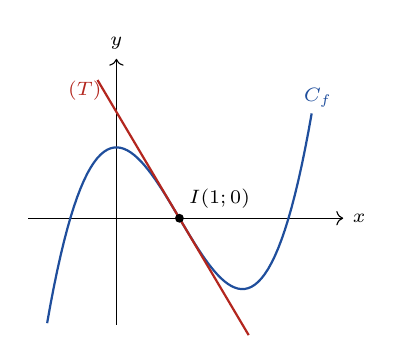
\begin{tikzpicture}[x=0.8cm,y=0.45cm,font=\scriptsize]
\draw[->] (-1.4,0)--(3.6,0) node[right]{$x$}; \draw[->] (0,-3)--(0,4.5) node[above]{$y$};
\draw[cDef,thick,domain=-1.1:3.1,samples=80] plot (\x,{\x*\x*\x-3*\x*\x+2}); \node[cDef] at (3.2,3.4){$C_f$};
\draw[cThm,thick,domain=-0.3:2.1] plot (\x,{-3*\x+3}); \node[cThm] at (-0.5,3.6){$(T)$};
\fill (1,0) circle (1.6pt) node[above right]{$I(1;0)$};
\end{tikzpicture}\end{LTR}\par }{50 د}{جدول إشارة $f^{\prime\prime}$.}
\Row{}{%
\Lab{cRem}{ملاحظات}\ إذا انعدمت $f^{\prime}$ عند $a$ دون أن تغير إشارتها فالنقطة أيضاً نقطة انعطاف (المماس أفقي).\par\Lab{cThm!80!black}{حذار}\ انعدام $f^{\prime\prime}$ وحده لا يكفي: $x^4$ عند $0$.}{}{}
\Row{التقويم}{%
\Lab{cEx}{تطبيق}\par عيّن نقط انعطاف منحني $f(x)=x^4-6x^2$.\par\textbf{الحل:} $f^{\prime\prime}(x)=12x^2-12=12(x-1)(x+1)$ يغير إشارته عند $\pm1$: النقطتان $(-1;-5)$ و $(1;-5)$.\par\textbf{واجب منزلي:} تمرين 67 صفحة 64 ، وتمرين 70 صفحة 65.\par\smallskip\textbf{ملاحظات حول سير الحصة:} \dotfill}{25 د}{تقويم فردي.}
\end{Sayr}
\newpage
\ModhHead{06}{3 ع ت}{تحليل}{الاشتقاقية والاستمرارية}{02 سا}{اتجاه التغير ، القيم الحدية ، التقريب التآلفي}%
{\begin{itemize}\item المشتقات ، القيم الحدية المحلية (2 ع ت).\end{itemize}}%
{\begin{itemize}\item دراسة اتجاه تغير دالة ، وتعيين قيمها الحدية.\item استعمال التقريب التآلفي لحساب قيم مقربة.\end{itemize}}%
{المنهاج ، الكتاب المدرسي ، مراجع ، الحاسبة البيانية.}
\begin{Sayr}
\Row{مرحلة الانطلاق}{%
\textbf{التهيئة النفسية:} بدون حاسبة: قيمة مقربة لـ $\sqrt{4{,}02}$ ؟}{10 د}{تحدٍّ ذهني.}
\Row{التشخيص والاكتشاف}{%
\Lab{cEx}{وضعية مقترحة}\par\ck\ $f(x)=\sqrt x$ عند $4$: $f(4+h)\approx f(4)+f^{\prime}(4)h=2+\dfrac h4$.\par
\ck\ $\sqrt{4{,}02}\approx2{,}005$ (الحاسبة: $2{,}00499$).\par
}{35 د}{مقارنة بالحاسبة.}
\Row{بناء المعارف}{%
\Lab{cThm}{اتجاه التغير}\ إشارة $f^{\prime}$ على مجال تعطي اتجاه تغير $f$ ؛ إذا انعدمت $f^{\prime}$ عند $a$ مغيرة إشارتها فـ $f(a)$ قيمة حدية محلية.\par\Lab{cThm}{التقريب التآلفي}\ من أجل $h$ قريب من $0$: $f(a+h)\approx f(a)+f^{\prime}(a)\,h$.\par}{50 د}{جدول التغيرات.}
\Row{}{%
\Lab{cEx}{مثال}\ $(1+h)^5\approx1+5h$: $1{,}003^5\approx1{,}015$.\par\Lab{cThm!80!black}{حذار}\ التقريب جيد فقط لـ $h$ صغير.}{}{}
\Row{التقويم}{%
\Lab{cEx}{تطبيق}\par $g(x)=x+\dfrac4x$ على $]0;+\infty[$. ادرس اتجاه تغيرها ، وعيّن قيمتها الحدية.\par\textbf{الحل:} $g^{\prime}(x)=\dfrac{x^2-4}{x^2}$: متناقصة على $]0;2]$ ، متزايدة على $[2;+\infty[$ ؛ قيمة حدية صغرى $g(2)=4$.\par\textbf{واجب منزلي:} تمارين 11 ، 12 ، 13 صفحتي 36 و 37.\par\smallskip\textbf{ملاحظات حول سير الحصة:} \dotfill}{25 د}{تقويم فردي.}
\end{Sayr}
\newpage
\ModhHead{07}{3 ع ت}{تحليل}{الاشتقاقية والاستمرارية}{02 سا}{توظيف المشتقات لحل مشكلات}%
{\begin{itemize}\item دراسة اتجاه التغير ، القيم الحدية.\end{itemize}}%
{\begin{itemize}\item دراسة دوال كثيرات حدود ، ناطقة ، صماء ، وحل مسائل استمثال.\end{itemize}}%
{المنهاج ، الكتاب المدرسي ، مراجع ، الحاسبة البيانية.}
\begin{Sayr}
\Row{مرحلة الانطلاق}{%
\textbf{التهيئة النفسية:} من صفيحة مربعة ضلعها $12$ cm نقطع مربعات في الأركان ونطوي: ما أكبر حجم للعلبة؟}{10 د}{مسألة من الحياة.}
\Row{التشخيص والاكتشاف}{%
\Lab{cEx}{وضعية مقترحة}\par\ck\ $x$ ضلع المربع المقطوع ، $0<x<6$: $V(x)=x(12-2x)^2$.\par
\ck\ $V^{\prime}(x)=12(x-2)(x-6)$: أكبر حجم $V(2)=128$ cm$^3$.\par
}{35 د}{عمل بالأفواج.}
\Row{بناء المعارف}{%
\Lab{cMeth}{حل مسألة استمثال}\ نختار المتغير ومجاله ، نعبر عن المقدار بدالة ، ندرس تغيراتها ، ونقرأ القيمة الحدية.\par\Lab{cEx}{دالة صماء}\ $f(x)=x\sqrt{4-x}$ على $[0;4]$: $f^{\prime}(x)=\dfrac{8-3x}{2\sqrt{4-x}}$ على $[0;4[$: متزايدة على $[0;\frac83]$ ومتناقصة على $[\frac83;4]$ ؛ القيمة العظمى $f(\frac83)=\dfrac{16\sqrt3}9$.\par}{50 د}{مخطط حل مسألة استمثال.}
\Row{}{%
\Lab{cThm!80!black}{حذار}\ نتحقق من أن القيمة الحدية تنتمي إلى المجال المقبول فيزيائياً.}{}{}
\Row{التقويم}{%
\Lab{cEx}{تطبيق}\par مستطيل مساحته $16$ cm$^2$. عيّن بعديه حتى يكون محيطه أصغر ما يمكن.\par\textbf{الحل:} $P(x)=2\left(x+\dfrac{16}x\right)$ ، $P^{\prime}(x)=2\dfrac{x^2-16}{x^2}$: أصغر محيط عند $x=4$: مربع ضلعه $4$ ، $P=16$ cm.\par\textbf{واجب منزلي:} تمارين من باب الاشتقاقية (مسائل).\par\smallskip\textbf{ملاحظات حول سير الحصة:} \dotfill}{25 د}{تقويم فردي.}
\end{Sayr}
\newpage
\ModhHead{08}{3 ع ت}{تحليل}{الاشتقاقية والاستمرارية}{02 سا}{دراسة الدوال المثلثية $x\mapsto\cos(\omega x+\varphi)$ و $x\mapsto\sin(\omega x+\varphi)$}%
{\begin{itemize}\item حساب المثلثات ، مشتق دالة مركبة.\end{itemize}}%
{\begin{itemize}\item حساب مشتقات الدوال المثلثية ، ودراسة دالة مثلثية على دور.\end{itemize}}%
{المنهاج ، الكتاب المدرسي ، مراجع ، الحاسبة البيانية.}
\begin{Sayr}
\Row{مرحلة الانطلاق}{%
\textbf{التهيئة النفسية:} ما دور الدالة $\sin$ ؟ وما دور $\sin(2x)$ ؟}{10 د}{سؤال.}
\Row{التشخيص والاكتشاف}{%
\Lab{cEx}{مناقشة نشاط 02 (أنشطة باب الاشتقاقية)}\par\ck\ نقطة على الدائرة المثلثية ، وتفسير هندسي لـ $\dfrac{\sin h}h$ لما $h\to0$.\par
\ck\ تخمين: $\sin^{\prime}=\cos$.\par
}{35 د}{نشاط الكتاب.}
\Row{بناء المعارف}{%
\Lab{cThm}{خاصية}\par\ck\ $\sin^{\prime}(x)=\cos x$ ، $\cos^{\prime}(x)=-\sin x$.\par
\ck\ $\big(\sin(\omega x+\varphi)\big)^{\prime}=\omega\cos(\omega x+\varphi)$ ، $\big(\cos(\omega x+\varphi)\big)^{\prime}=-\omega\sin(\omega x+\varphi)$.\par
\ck\ الدالتان دوريتان ودورهما $\dfrac{2\pi}{|\omega|}$.\par
\Lab{cMeth}{دراسة دالة مثلثية}\ نعين الدور ، والشفعية ، ثم ندرس الدالة على مجال طوله دور (أو نصف دور) ونستنتج المنحني بالانسحاب والتناظر.\par}{50 د}{منحني على دور ثم الانسحاب.}
\Row{}{%
\Lab{cEx}{مثال}\ $f(x)=\sin2x$: الدور $\pi$ ، فردية ؛ $f^{\prime}(x)=2\cos2x$: متزايدة على $[0;\frac\pi4]$ ، متناقصة على $[\frac\pi4;\frac{3\pi}4]$ ، متزايدة على $[\frac{3\pi}4;\pi]$.\par\Lab{cThm!80!black}{حذار}\ $\omega$ يظهر عاملاً في المشتقة.}{}{}
\Row{التقويم}{%
\Lab{cEx}{تطبيق}\par $f(x)=\cos\left(3x-\frac\pi2\right)$. بسّط $f(x)$ ، عيّن دورها ، واحسب $f^{\prime}(x)$.\par\textbf{الحل:} $f(x)=\sin3x$ ، الدور $\dfrac{2\pi}3$ ، $f^{\prime}(x)=3\cos3x$.\par\textbf{واجب منزلي:} تمرين 63 صفحة 69 ، وتمرين 95 صفحة 70.\par\smallskip\textbf{ملاحظات حول سير الحصة:} \dotfill}{25 د}{تقويم فردي.}
\end{Sayr}
\newpage
\ModhHead{09}{3 ع ت}{تحليل}{الاشتقاقية والاستمرارية}{02 سا}{المعادلات التفاضلية $y^{\prime}=f$}%
{\begin{itemize}\item مشتقات الدوال المألوفة.\end{itemize}}%
{\begin{itemize}\item حل معادلات تفاضلية من الشكل $y^{\prime}=f(x)$ ، وتعيين الحل الذي يحقق شرطاً ابتدائياً.\end{itemize}}%
{المنهاج ، الكتاب المدرسي ، مراجع ، الحاسبة البيانية.}
\begin{Sayr}
\Row{مرحلة الانطلاق}{%
\textbf{التهيئة النفسية:} نعرف سرعة سيارة في كل لحظة: هل نستطيع معرفة المسافة المقطوعة؟}{10 د}{سؤال فيزيائي.}
\Row{التشخيص والاكتشاف}{%
\Lab{cEx}{وضعية مقترحة}\par\ck\ $y^{\prime}=2x$: الدوال $x^2$ ، $x^2+1$ ، $x^2-5$ كلها حلول.\par
\ck\ لتعيين حل وحيد نحتاج شرطاً ، مثلاً $y(0)=3$.\par
}{35 د}{نبحث عن «الدالة الأصلية».}
\Row{بناء المعارف}{%
\Lab{cDef}{تعريف}\ حل المعادلة $y^{\prime}=f(x)$ على $I$ هو كل دالة $F$ قابلة للاشتقاق على $I$ حيث $F^{\prime}=f$.\par\Lab{cThm}{خاصية}\ إذا كانت $F$ حلاً فالحلول هي الدوال $x\mapsto F(x)+c$ ($c$ ثابت حقيقي) ، ويوجد حل وحيد يحقق $y(x_0)=y_0$.\par}{50 د}{نتحقق بالاشتقاق.}
\Row{}{%
\Lab{cEx}{مثال}\par\ck\ $y^{\prime}=3x^2-2x$: $y=x^3-x^2+c$ ؛ مع $y(1)=2$: $c=2$.\par
\ck\ $y^{\prime}=\cos2x$: $y=\frac12\sin2x+c$.\par
\Lab{cThm!80!black}{حذار}\ لا ننسى الثابت $c$.}{}{}
\Row{التقويم}{%
\Lab{cEx}{تطبيق}\par حل على $]0;+\infty[$: $y^{\prime}=\dfrac1{x^2}$ ، ثم عيّن الحل الذي يحقق $y(1)=0$.\par\textbf{الحل:} $y=-\dfrac1x+c$ ؛ $-1+c=0$ ، $c=1$: $y=1-\dfrac1x$.\par\textbf{واجب منزلي:} تمارين من باب الاشتقاقية.\par\smallskip\textbf{ملاحظات حول سير الحصة:} \dotfill}{25 د}{نهاية المحور: فرض أو مراجعة.}
\end{Sayr}
\end{document}
